%\documentclass[tip_rada, jezik]{FSBtex}
% moguce opcije su:
%	-> tip_rada: seminar, zavrsni, projekt, diplomski
%	-> jezik (dodatni parametar, moze i bez njega ako se pise na hrvatskom): hrvatski, engleski
\documentclass[disertacija,hrvatski]{FSBtex}


\usepackage{lipsum}

% naredbe za generiranje datoteke
% pdflatex main.tex
% bibtex main
% makeindex -s nomencl.ist -o main.nls main.nlo
% makeglossaries-lite main
% pdflatex main.tex
% pdflatex main.tex

 

%----------------------------------------------------------------------------------------
%	POSTAVKE RADA
%----------------------------------------------------------------------------------------

\title{Naslov disertacije test HR}
\titleENG{Title dissertation test ENG}

\author{Marko Markić}

\mentor{prof. dr. sc. Miki Mikić, dip. ing.}
\mentorDva{dr. sc. Pero perić, dip. ing.}
\mentorENG{Full prof. Miki Mikić, PhD}
\mentorDvaENG{Associate prof. Pero perić, PhD}


%-- sljedeci elementi potrebni su za doktorsku disertaciju:



\zahvala{
Izjavljujem da sam ovaj rad izradio samostalno koristeći stečena znanja tijekom studija i navedenu literaturu.\\

Zahvaljujem se svom mentoru \textbf{prof. dr. sc. Peri Periću} što mi je omogućio da napišem ovaj rad......
}


\zadatak{slike/zadatak.pdf}

\keywordsHR{PID; LQR; hidraulika}
\keywordsENG{PID; LQR; hydraulics}

%----------------------------------------------------------------------------------------
%	POCETAK DOKUMENTA
%----------------------------------------------------------------------------------------
\begin{document}
		
\NaslovnaStrana	% ova naredba ukljucuje sve naslovne strane rada ovisno o tipu rada, te sadrzaj i popise slika i tablica
	
\newpage
\clearpage
\ifpdf
\phantomsection
\fi
\pagestyle{empty}
\begin{center}
	\textbf{\large Supervisor Information}
\end{center}


\begin{flushleft}
Profesor Profesor, PhD, Associate Professor\\
Department of Robotics and Production System Automation\\
Faculty of Mechanical Engineering and Naval Architecture, University of Zagreb\\
Croatian scientist ID: xxxxxx

%\url{https://scholar.google.hr/citations?user=EYo5QcMAAAAJ}

\end{flushleft}


Lorem ipsum dolor sit amet, consectetur adipiscing elit, sed do eiusmod tempor incididunt ut labore et dolore magna aliqua. Metus aliquam eleifend mi in nulla posuere sollicitudin aliquam ultrices. Nibh praesent tristique magna sit amet. Posuere morbi leo urna molestie at elementum eu facilisis. Ipsum dolor sit amet consectetur adipiscing elit pellentesque. Posuere sollicitudin aliquam ultrices sagittis orci a scelerisque purus. Rhoncus mattis rhoncus urna neque viverra justo nec. Egestas purus viverra accumsan in nisl nisi scelerisque eu ultrices. Tellus in metus vulputate eu scelerisque. Convallis posuere morbi leo urna molestie at elementum eu facilisis. Vivamus at augue eget arcu dictum varius. Varius duis at consectetur lorem donec massa sapien faucibus. Iaculis at erat pellentesque adipiscing commodo elit at. Est sit amet facilisis magna etiam tempor orci eu. Aenean euismod elementum nisi quis eleifend quam adipiscing vitae. Consequat interdum varius sit amet mattis vulputate enim nulla. Malesuada bibendum arcu vitae elementum. Ornare aenean euismod elementum nisi quis eleifend quam adipiscing vitae. Tellus in metus vulputate eu scelerisque felis imperdiet proin fermentum. Semper risus in hendrerit gravida.

Ac odio tempor orci dapibus. Ac odio tempor orci dapibus ultrices in iaculis nunc sed. Feugiat nibh sed pulvinar proin gravida hendrerit lectus. Molestie ac feugiat sed lectus vestibulum. Ornare arcu dui vivamus arcu felis bibendum ut tristique. Facilisis sed odio morbi quis commodo odio aenean sed adipiscing. Nibh venenatis cras sed felis eget velit aliquet sagittis id. Quam lacus suspendisse faucibus interdum posuere lorem ipsum. In mollis nunc sed id semper. Purus non enim praesent elementum facilisis leo vel fringilla est. Ac tincidunt vitae semper quis lectus nulla at volutpat diam. Turpis massa sed elementum tempus egestas. At quis risus sed vulputate odio ut enim blandit volutpat. Sem fringilla ut morbi tincidunt augue. Tristique risus nec feugiat in.

Dictumst vestibulum rhoncus est pellentesque elit ullamcorper. Orci porta non pulvinar neque laoreet. Neque ornare aenean euismod elementum nisi quis eleifend quam. Quis eleifend quam adipiscing vitae proin. Consequat ac felis donec et odio pellentesque diam volutpat commodo. Pellentesque elit eget gravida cum sociis natoque penatibus. Tortor condimentum lacinia quis vel eros. Pulvinar neque laoreet suspendisse interdum consectetur libero. Senectus et netus et malesuada fames. Pharetra et ultrices neque ornare. Condimentum id venenatis a condimentum vitae sapien pellentesque. Sit amet mattis vulputate enim nulla. Aenean sed adipiscing diam donec adipiscing tristique risus. Feugiat vivamus at augue eget arcu dictum. Amet justo donec enim diam vulputate ut. Ipsum dolor sit amet consectetur adipiscing elit pellentesque habitant. Eget mi proin sed libero enim sed faucibus turpis in. Turpis cursus in hac habitasse.


\newpage
\clearpage
\ifpdf
\phantomsection
\fi
\pagestyle{empty}
\begin{center}
	\subsection*{Acknowledgement}
\end{center}


I would like to give extensive thanks to my esteemed supervisor professor Lorem ipsum dolor sit amet, consectetur adipiscing elit, sed do eiusmod tempor incididunt ut labore et dolore magna aliqua. Metus aliquam eleifend mi in nulla posuere sollicitudin aliquam ultrices. Nibh praesent tristique magna sit amet. Posuere morbi leo urna molestie at elementum eu facilisis. Ipsum dolor sit amet consectetur adipiscing elit pellentesque. Posuere sollicitudin aliquam ultrices sagittis orci a scelerisque purus. Rhoncus mattis rhoncus urna neque viverra justo nec. Egestas purus viverra accumsan in nisl nisi scelerisque eu ultrices. Tellus in metus vulputate eu scelerisque. Convallis posuere morbi leo urna molestie at elementum eu facilisis. Vivamus at augue eget arcu dictum varius. Varius duis at consectetur lorem donec massa sapien faucibus. Iaculis at erat pellentesque adipiscing commodo elit at. Est sit amet facilisis magna etiam tempor orci eu. Aenean euismod elementum nisi quis eleifend quam adipiscing vitae. Consequat interdum varius sit amet mattis vulputate enim nulla. Malesuada bibendum arcu vitae elementum. Ornare aenean euismod elementum nisi quis eleifend quam adipiscing vitae. Tellus in metus vulputate eu scelerisque felis imperdiet proin fermentum. Semper risus in hendrerit gravida.

Ac odio tempor orci dapibus. Ac odio tempor orci dapibus ultrices in iaculis nunc sed. Feugiat nibh sed pulvinar proin gravida hendrerit lectus. Molestie ac feugiat sed lectus vestibulum. Ornare arcu dui vivamus arcu felis bibendum ut tristique. Facilisis sed odio morbi quis commodo odio aenean sed adipiscing. Nibh venenatis cras sed felis eget velit aliquet sagittis id. Quam lacus suspendisse faucibus interdum posuere lorem ipsum. In mollis nunc sed id semper. Purus non enim praesent elementum facilisis leo vel fringilla est. Ac tincidunt vitae semper quis lectus nulla at volutpat diam. Turpis massa sed elementum tempus egestas. At quis risus sed vulputate odio ut enim blandit volutpat. Sem fringilla ut morbi tincidunt augue. Tristique risus nec feugiat in.


\begin{abstract}

	  are categorized as autonomous or remotely controlled aircraft that hold a many favourable features allowing them a wide range of useful applications. In order to successfully complete a flight mission, the aircraft must comply with the required flight performance indices. Aircraft performance depends strongly on the propulsion system and therefore different flight characteristics require different propulsion implementations. In contrast to well–known benefits of   utilisation, in particular multirotor type of  there is one major drawback regarding the on–board available energy. Most common electrically powered aircraft can last in the air for 15 to 30 minutes, while the best ones may last up to 60 minutes.
	
	Therefore, to overcome the aforementioned drawbacks of purely–electric energy source in multirotor aircraft, alternative propulsion systems combining two different energy sources (hybrid power systems) are considered.
	In this work, a methodological approach to the design of a hybrid propulsion unit for multirotor aircraft consisting of an internal combustion engine, electricity generator and electrochemical battery is described.
	
	For this purpose, analysis and modelling of individual components of the propulsion system have been carried out. Physical parameters of dynamic models are identified by means of experimental measurements. Based on the obtained data, a detailed model of a hybrid electrical propulsion configuration was proposed and suitable control strategies for the hybrid power system have been designed. The proposed control system design methodology has been verified by exhaustive computer simulations and experimentally by using different experimental setups. 
\end{abstract}


% \begin{prosirenisazetak}

	Bespilotne letjelice s više rotora pripadaju u kategoriju autonomnih ili daljinski upravljanih zrakoplova karakteriziranih nizom svojstava koje im omogućuju širok raspon korisnih primjena. U svrhu uspješnog ispunjenja letačke misije, letjelica mora zadovoljiti tražene performanse. Uporabljivost takvih letjelica uvelike ovisi o pogonskom sustavu, te zbog toga letački zadaci različitih profila zahtijevaju različite vrste i konfiguracije pogona, sposobnosti vertikalnog polijetanja i slijetanja, \textit{engl.} \{vtol}, kao i održavanja stacionarnih i sporih letova. Letjelice ovog tipa imaju širok raspon korisnih primjena, kao što je podrška iz zraka prilikom nadgledanja, pomoć kod katastrofa ili misija traženja i spašavanja, granične patrole i detekcije neovlaštene prisutnost uz otkrivanje upada i slično. Moderne višerotorske letjelice se sve više koriste u rekreativne i natjecateljske uloge kao što su utrke, snimanje iz zraka uključujući trodimenzijsko skeniranje objekata ili terena, te u poljoprivredne svrhe poput kontrole rasta vegetacije i kontrole utjecaja štetočina. 
	
	Zahvaljujući ubrzanom razvoju sastavnih komponenti poput senzorskog sustava, mikrokontrolera, te pogona i baterija, danas su dostupne različite višerotorske letjelice bazirane na „software“–u i „hardwareu“–u otvorenog koda. Takve letjelice prikladne su za istraživanje i ispitivanje različitih regulacijskih sustava stabilizacije leta.		
	Međutim, dinamika takvih sustava je inherentno  nestabilna, što znači da letjelica ne zadržava zadanu putanju, osim ako se ne primjenjuju stabilizacijske akcije. Letjelicu karakterizira šest stupnjeva slobode gibanja (tj. tri translacije i tri rotacije), dok je njena dinamika nelinearna. Također, sustav može biti pod–upravljan ukoliko konfiguracija pogonskog sustava ne omogućava neovisno gibanje za svaki stupanj slobode, odnosno drugim riječima, ako se rotacijsko i translacijsko gibanje vozila ne može razdvojiti na nezavisne komponente. 
	
	Veliki nedostatak je ograničeno vrijeme leta od obično 15–60 minuta (autonomija) i ograničenja nosivosti korisnog tereta, pri čemu je povećanje veličine tereta u korelaciji sa kraćim vremenom trajanja leta. Određena poboljšanja autonomije više–rotorskih bespilotnih letjelica dobivena su korištenjem motora s unutarnjim izgaranjem kao glavnim pogonom propelera. Za takve sustave, glavni problem je kada letjelica zahtijeva brzu i preciznu kontrolu brzine vrtnje propelera kako bi se postigao željeni profil leta, gdje dinamika motora s unutrašnim izgaranjem potencijalno nije dovoljno brza.
	
	Pogonski sustav letjelice ključan je i neophodan modul koji ima zadatak osigurati stalni potisak propelera kako bi se održao stabilan let. Performanse, učinkovitost i korisnost letjelice značajno ovise o pogonskim karakteristikama i mogućnostima. Tipičan pogon sastoji se od većeg broja propelera spojenih na odgovarajuće pogonske motore koji rotacijom generiraju okretni moment a posljedično i potisak propelera. Pritom izvedbe mogu biti s fiksnim ili varijabilnim kutom propelera, koaksijalno montirani i montirani pod kutem. U literaturama je pokazano da svaki izbor konfiguracije pogonskog sustava ima značajan utjecaj na ponašanje letjelice. Za potrebe održavanja stabilnog lebdećeg položaja, minimalni zahtjev je ostvarenje neto sile potiska koja je približno jednaka težini letjelice. U praksi se pokazalo da bi omjer ukupne potisne sile propelera i težine letjelice, \textit{engl.} \ {twr} trebao bi biti okvirno dva ili više kako bi se osiguralo dovoljno snage za zadovoljavajuće performanse letjelice.

	Propeleri su učestalo pogonjeni električnim motorima s elektroničkom komutacijom, trapeznih oblika elektormotorne sile, \textit{engl.} \ {bldc} ili sinusoidalnih oblika elektromotorne sile, \textit{engl.} \ {pmsm} koji su opremljeni odgovarajućim regulatorima brzine vrtnje. U većini slučajeva vratilo motora izravno je spojeno s propelerom bez prijenosnog mehanizma (tj. zupčanog ili lančanog pogona). Premda je \ {bldc} odnosno \ {pmsm} motor složeniji za analizu prilikom sinteze sustava upravljanja, posjeduje povoljnija svojstva od istosmjernog motora s četkicama i mehaničkim komutatorom, \textit{engl.} \ {dc}  Machine zbog veće učinkovitosti u pretvorbi električne u mehaničku energiju i niskih zahtjeva za održavanjem. \ {bldc} i \ {pmsm} motori obično su pogonjeni pravokutno oblikovanim faznim naponom kroz šest koraka komutacije. U naprednijim strukturama koristi se i vektorsko upravljanje, posebice za \ {pmsm}.

	Trofazna armatura može biti spojena u zvijezdu (wye) ili trokut (delta) konfiguraciju namota. Pojednostavljeni ekvivalentni model \ {uav} motora može se izvesti u svrhu analize i modeliranja dinamike pogonskog sustava.

	Elektrokemijske baterije rašireno se koriste kao izvor napajanja više–rotorskih letjelica. Litij–polimerne, \textit{engl.} \ {lipo} baterije u upotrebi su zbog velike gustoće energije, mogućnosti isporuke značajne snage u kratkim vremenskim intervalima i relativno male mase te predstavljaju najčešću vrstu izvora energije za pogon \ {uav} letjelica, imajući pritom značajne prednosti nad Nikal–Metalnim Hibridnim, \textit{engl.} \ {nimh} baterijama u smislu gustoće energije. Međutim, čak i moderne baterije ne mogu osigurati dovoljno energije za dulje letačke misije. Stoga treba istražiti alternativne izvore energije kako bi se povećala autonomija, primjerice primjenu motora s unutarnjim izgaranjem i električnim generatorom i moguće kombinacije s baterijom kao pomoćnim izvorom energije. Kako bi se procijenila preostala zaliha energije baterije, potrebno je pratiti njeno stanje napunjenosti, \textit{engl.} \ {soc}.

	Važna komponenta koji omogućuje stabilan let je regulacijski sustav, budući da se letjelica ne može sama stabilizirati bez održavanja upravljačkih komandi za električne motore. Glavni zadatak regulatora je tumačenje ulaznih signala te generiranje izlaznih signala kako bi svaki motor mogao postići traženu brzinu vrtnje. Uobičajeno se sinteza upravljačkih algoritama temelji na pojednostavljenom modelu dinamike tijela zanemarujući složenu dinamiku motora i propelera. Vanjske sile i momenti koje generira pogon su ulazi u sustav dok je orijentacija letjelice definirana tzv. Eulerovim kutovima. 
	
	Ovo doktorsko istraživanje opisuje metodološki pristup dizajniranju upravljačkih sustava više–rotorske letjelice sa hibridno–električnom pogonskom jedinicom, temeljenim na kombinaciji motora sa unutrašnjim izgaranjem, električnog generatora i elektrokemijske baterije. Nadalje, izvršena je analiza i modeliranje pojedinih komponenata hibridnog pogonskog sustava. Fizički parametri dinamičkih modela komponenata pogona identificirani su mjerenjima na izgrađenim odgovarajućim eksperimentalnim postavima. Na temelju dobivenih podataka predložen je detaljan model dinamike hibridnog pogonskog sustava za dvije odabrane konfiguracije izvora energije. Predložena metodologija verificirana je računalnim simulacijama i na izgrađenim eksperimentalnim postavima.

	U sklopu Laboratorija za elektrotehniku izgrađeni su sljedeći eksperimentalni postavi:

	\begin{itemize}

		\item Laboratorijski postav za ispitivanje agregata u sklopu hibridnog sustava propulzije bespilotne letjelice zasnovanog na motoru s unutarnjim izgaranjem i generatorom temeljenom na beskolektorskom istosmjernom stroju, sa paralelno dodatnom elektrokemijskom baterijom. 

		
		\item Laboratorijski postav za ispitivanje sustava upravljanja tokovima električne energije temeljenog na DC-DC energetskim pretvaračima i litij–polimernim baterijama. 

		
		\item Laboratorijski postav za ispitivanje propelerskih potisnika (propulzora) u sklopu sustava hibridne propulzije.

	\end{itemize}

	Nakon izgradnje navedenih eksperimentalnih postava proveden je niz mjerenja kojima su identificirani matematički modeli namijenjeni sintezi sustava upravljanja hibridnom propulzijom bespilotne letjelice, odnosno provedena je eksperimentalna provjera odgovarajućuh sustava upravljanja hibridnim pogonom letjelice. Time su postignuti glavni ciljevi istraživanja, odnosno: 

	\begin{itemize}

		\item Razrađen je sustavni pristup modeliranju dinamike hibridnog pogonskog sustava više–rotorskih bespilotnih letjelica. 

		
		\item Temeljem dobivenog dinamičkog modela hibridnog pogonskog sustava i odgovarajućeg postupka sinteze upravljačkog sustava dobivena su poboljšanja u performansama sustava propulzije letjelice.

	\end{itemize}

	Provedena istraživanja rezultirala su znanstvenim doprinosima koji se mogu sažeti kako slijedi:

	\begin{itemize}

		\item Identificirani su matematički modeli pojedinih komponenti pogonskog sustava hibridne višerotorske bespilotne letjelice u svrhu dobivanja sveobuhvatnog dinamičkog modela pogonskog sustava, s ciljem poboljšanja procesa sinteze upravljačkog sustava pogona i letjelice.

		
		\item 	Razrađen je postupak projektiranja upravljačkog sustava pogona hibridne letjelice koji uključuje dinamičke karakteristike i eksperimentalno je potvrđen razvijeni sustavni pristup projektiranju regulacijskog sustava hibridne propulzije i letjelice, temeljen na matematičkom modelu koji uključuje dinamičke karakteristike hibridnog pogonskog sustava, čime se u konačnici postižu poboljšane performanse cjelokupnog sustava upravljanja dinamikom letjelice.

	\end{itemize}

	Istraživanje prikazano u ovome radu podijeljeno je u šest faza, koje ga opisuju kako slijedi:

	\begin{enumerate}

		\item \textit{Analiza dinamike i modeliranje pojedinih komponenata hibridnog pogonskog sustava}\\
		U prvoj fazi provodi se matematičko modeliranje sastavnih komponenti pogona hibridne letjelice, koje su međusobno povezane i na različite načine pridonose dinamici letjelice. Kako bi se istražio cijeli raspon dinamike pogonskog sustava, istu je potrebno podijeliti na elementarne komponente i provesti temeljitu analizu, koristeći pritom odgovarajuće fizikalne zakonitosti za opisivanje značajki pogona, na temelju čega se razvijaju dinamički modeli koji su pogodni za računalne simulacije

		
		\item \textit{Eksperimentalna mjerenja i identifikacija fizikalnih konstanti} \\
	Za potrebe razvoja odgovarajućih dinamičkih modela komponenata pogonskog sustava letjelice, na izgrađenim postavima provode se eksperimentalana mjerenja za identifikaciju fizikalnih konstanti. Snimanje rezultata ostvareno je povezivanjem senzorskog sustava s računalom pomoću odgovarajućeg sučelja za prikupljanje signala u realnom vremenu i spremanje prodataka za naknadnu analizu na računalu. 

		
		\item \textit{Razvoj modela hibridnog pogonskog sustava letjelice} \\
		Koristeći prethodno dobivene modele pogonskih podsustava postavlja se model pogona na kojem se temelji sinteza regulacijskog sustava hibridnog pogona letjelice. Također, predlaže se sveobuhvatni model hibridne propulzije za dvije konfiguracije razmatrane u ovom radu.

		
		\item \textit{Implementacija sustava upravljanja hibridnom propulzijom} \\  
		Eksperimentalna implementacija razvijenih upravljačkih algoritama izvodi se na  mikrokontrolerskom sustavu čije je programiranje podržano unutar Matlab/Simulink™ programskog okruženja koje omogućuje generiranje i učitavanje odgovarajućeg programskog koda. 

		
		\item \textit{Eksperimentalna validacija predložene metode}\\
		Za razvijenu metodologiju sustavi upravljanja hibridnim pogonom letjelice ispituju se u realnim uvjetima rada, koristeći pritom izgrađene eksperimentalne postave.

		
		\item \textit{Završetak} \\
		Izvedba zaključaka iz provedenih istraživanja. Prikupljanje rezultata i analiza znanstvenog doprinosa, objavljivanje znanstvenih radova.

		
	\end{enumerate}

	
	
	
\end{prosirenisazetak}


	% sadrzaj, popis slika, tablica, oznaka...
\sadrzaj

% sve sa A se prvo ispisuje kod oznaka

%% OVO NE RADI!!! +

%\nomenclature[A]{$s$}{klizna površina SMC regulatora \nomunit{\si{\kilogram\per\cubic\meter}}}
%\nomenclature[A]{$k_1,\ k_2$}{pojačanja SMC regulatora \nomunit{-}}%
%\nomenclature[A]{$k_1,\ k_2,\ k_3$}{pojačanja metode povratnog koraka \nomunit{-}}%
%
%% konstante
%\nomenclature[C]{$g$}{gravitacijsko ubrzanje  \nomunit{9,81 \si{\meter\per\square\second}}}%
%
%%% grcke oznake
%\nomenclature[G]{$\beta,\ \gamma$}{težinski koeficijenti PID regulatora \nomunit{-}}%
%\nomenclature[G]{$\rho$}{gustoća fluida, \nomunit{\si{\kilogram\per\cubic\meter}} }%
%
%% indeksi
%\nomenclature[I]{$\alpha_d$}{koeficijent istjecanja \nomunit{-}}%
%
%% akcenti
%\nomenclature[T]{$\underline{\square}$}{Dual quaternion }%
%
%% kratice
%\newacronym{ga}{GA}{genetski algoritmi (eng. \textit{Genetic Algorithms})}
% 
 
 %% OVO NE RADI!!! -

 
 
%----------------------------------------------------------------------------------------
%	OVDJE IDE OSTATAK RADA I SVA POGLAVLJA
%----------------------------------------------------------------------------------------
% pocetak brojanja rada od prve stranice
\pagebreak
\setcounter{page}{1}
\pagenumbering{arabic}

% ovdje ide ostatak rada
\chapter{Uvod}
Jedan od najznačajnijih problema kod konstruiranja mehanizama je optimalna sinteza mehanizma.
Tijekom godina razvijeno je nekoliko metoda za sintezu mehanizama \cite{Chiang2000, Hansen2009} ali svaka od njih primjenjiva je samo na određenim tipovima mehanizma. 
Zbog toga odabir odgovarajuće metode optimiranja mehanizma ovisi o samom mehanizmu koji se želi optimirati tj. aplikaciji mehanizma, potrebnoj numeričkoj točnosti te vremenu koje je potrebno da se postigne optimalno riješenje.

Primjena mehanizma utječe na optimizacijski problem, tj. ograničuje ga. U industrijskim aplikacijama ta ograničenja su dužine elemenata, prostor u koji mehanizam mora stati...\\

Možemo razlikovati dvije vrsta optimalne sinteze mehanizma: dimenzionalna i strukturalna sinteza. 
Dimenzionalna sinteza svodi se na određivanje dimenzija linkova mehanizma koji će omogućiti slijeđenje željene trajektorije ili funkcije, dok su mehanizam i veze između linkova poznati.
Strukturalna sinteza teži je problem jer nam nije poznat mehanizam ni veze između linkova te stoga moramo optimirati i topologiju i dimenzije mehanizma.\\

U ovom radu koristiti će se \acrlong{ga} ili \acrshort{ga} \cite{McCall2005, Cabrera2002} za optimiranje mehanizma.
Referenca na primjer tablice~\ref{tbl:primjer}.


\begin{table}[h!]
\centering
\caption{Primjer tablice}
\label{tbl:primjer}
\begin{tabular}{ccc}
stupac 1 & stupac 2 & stupac 3\\
\hline
\hline
nesto & $a+b$ & nesto\\
$a+b$ & nesto & $a+b$\\
\hline
\end{tabular}
\end{table}
\chapter{Izvod matematičkog modela}

Za mehanizam sa slike \ref{fig:mehanizma} potrebno je izvršiti optimalnu sintezu dimenzija mehanizma tako da bi moment na ručici $A_0A$ bio konstantan. U cilindru se nalazi idealni plin i cijeli proces se odvija pri konstantnoj temperaturi. Zadane su slijedeće vrijednosti:
\begin{align*}
h_1&=250\ \text{mm}\\
h_2&=75\ \text{mm}\\
F_1&=18\ \text{N}\\
\Delta \varphi &=\frac{\pi}{3}\\
A&=konst
\end{align*}

\begin{figure}[H]
\center
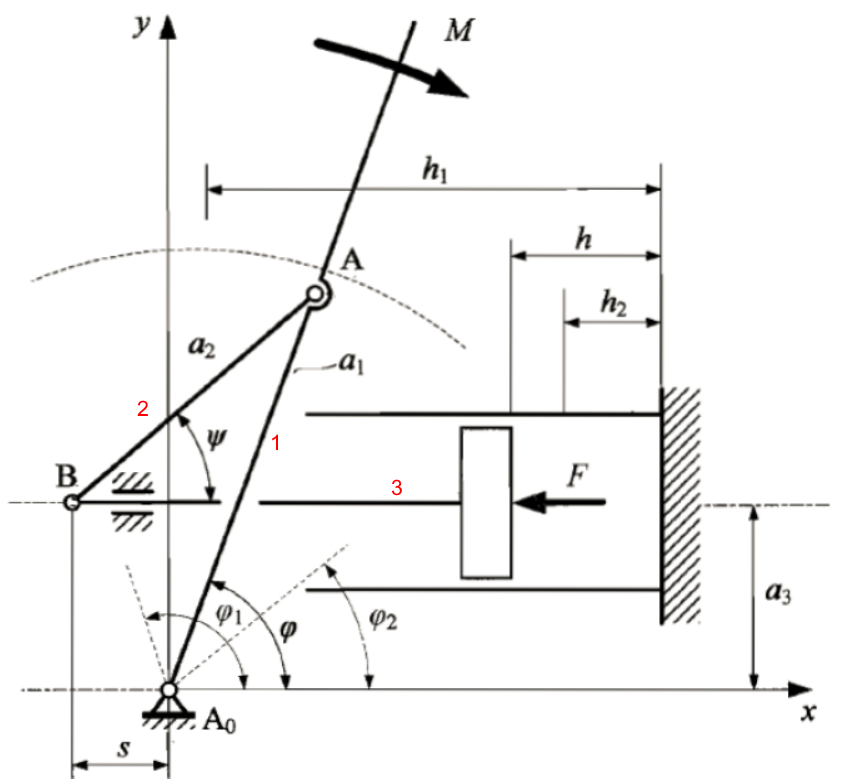
\includegraphics[scale=.4]{slike/mehanizam.png}
\caption{Skica mehanizma za optimiranje}
\label{fig:mehanizma}
\end{figure}

\section{Izvod funkcije cilja}
\quad Za konstantu temperaturu i eksponent politrope $n=1$ dobivamo ravnotežnu promjenu stanja kod koje se temperatura radnog medija ne mijenja tj. $T_1=T_2=T$ i $\Delta T=0$.\\

Jednadžbe stanja:
\begin{equation}
\label{eq:stanje1}
p_1V_1=mRT_1
\end{equation}
\begin{center}
i
\end{center}
\begin{equation}
\label{eq:stanje2}
p_2V_2=mRT_2
\end{equation}

povezane uvjetom $T_1=T_2=T$ daju sljedeću jednadžbu stanja:
\begin{equation}
\label{eq:stanje}
p_1V_1=p_2V_2=pV
\end{equation}

Volumen u cilindru računa se prema formuli \ref{eq:volumen} dok se sila na klip računa po izrazu \ref{eq:sila}.
\begin{equation}
\label{eq:volumen}
V=Ah
\end{equation}
\begin{equation}
\label{eq:sila}
F=pA
\end{equation}

Uvrstimo li izraze \ref{eq:volumen} i \ref{eq:sila} u jednadžbu \ref{eq:stanje} dobije se slijedeća jednadžba:
\begin{gather}
\dfrac{F_1}{A}h_1A=\dfrac{F_2}{A}h_2A=\dfrac{F}{A}hA\\
\label{eq:sile_polozaj}
F_1h_1=F_2h_2=Fh
\end{gather}

Iz zadanih vrijednosti i izraza \ref{eq:sile_polozaj} možemo izračunati silu $F_2$ (\ref{eq:F2}) te općeniti izraz za silu u ovisnosti o položaju klipa (\ref{eq:F}).
\begin{gather}
F_2=F_1\dfrac{h_1}{h_2}=18\dfrac{250}{75}\\
\label{eq:F2}
F_2=60\ N\\
\nonumber \\
F=F_1\dfrac{h_1}{h}=18\dfrac{250}{h}\\
\label{eq:F}
F=\dfrac{4500}{h}\ \text{N/mm}
\end{gather}

Nakon što smo dobili općeniti izraz za silu u ovisnosti o položaju možemo izraziti moment o ovisnosti o sili i položaju klipa preko elementarnih radova:
\begin{equation}
Md\varphi + Fdh=0
\end{equation}
\begin{equation}
M=-F\dfrac{dh}{d\varphi }=-\dfrac{4500}{h}\dfrac{dh}{d\varphi}
\end{equation}


Redukcijom sile na prvi član mehanizma (slika \ref{fig:mehanizma}) dobije se reducirani moment
\begin{equation}
\label{eq:reducirani}
M_{red}=F\dfrac{dh}{d\varphi }=\dfrac{4500}{h}\dfrac{dh}{d\varphi }
\end{equation}
tj. treba biti $M+M_{red}=0$.\\

Zbog toga traži se minimalno odstupanje funkcije $M(\varphi)=\dfrac{4500}{h}\dfrac{dh}{d\varphi }$ pri gibanju od $\varphi_1$ do $\varphi_2$.
Pomoću zadanog područja gibanja $\delta\varphi$ možemo izračunati konstantni moment:
\begin{gather}
d\varphi=\dfrac{4500}{M(\varphi )}\dfrac{dh}{h}\\
\nonumber\\
\varphi_1 - \varphi_2=\dfrac{4500}{M(\varphi)}ln\left(\dfrac{h_1}{h_2}\right)\\
\nonumber\\
M_{konst}=\dfrac{3\cdot 4500}{\pi}ln\left(\dfrac{250}{75}\right)=5173,69\ \text{Nmm}
\end{gather}

U ovom slučaju nam je zadatak minimizirati funkciju cilja $f(\varphi)=M(\varphi)-M_{konst}$.


\section{Kinematika mehanizma}

\quad Kinematička shema mehanizma s ishodištem koordinatnog sustava u točki $A_0$ prikazana je na slici \ref{fig:mehanizma}. Kod kinematičke analize mehanizma važno je unaprijed definirati koordinatni sustav i u skladu s njim paziti na predznake pomaka, sila idt. \\
Na osnovi kinematičkog modela sastavlja se matematički model za računanje kinematičkih veličina potrebnih za optimizaciju. To su položaj klipa $s$ odnosno $h$, kut $\varphi$ i derivacija $ds/dh=dh/d\varphi$.\\

Računanje položaja klipa $s$ pomoću prijenosnih funkcija mehanizma:
\begin{gather}
a_1sin(\varphi)+a_2sin(180+\psi)-a_3=0\\
\nonumber \\
sin(\psi) = \dfrac{a_1}{a_2}sin(\varphi)-\dfrac{a_3}{a_2}\\
\nonumber \\
sin(\psi) = k_1sin(\varphi)-k_2\\
\end{gather}
gdje su:
\begin{itemize}
\item $a_1=\sqrt{A_x^2+A_y^2}$
\item $a_2=\sqrt{(A_x-B_x)^2+(A_y-B_y)^2} $
\item $\varphi=atan\left( \dfrac{A_y}{A_x}\right) $
\item $k_1=\dfrac{a_1}{a_2}$
\item $k_2=\dfrac{a_3}{a_2}$
\end{itemize}

\begin{gather}
a_1cos(\varphi)+a_2cos(180^\circ+\psi)+scos(0)=0\\
\nonumber \\
s = a_2cos(\psi)-a_1cos(\varphi)\\
\nonumber \\
\label{eq:s}
s = -a_1cos(\varphi)+a_2\sqrt{1-(k_1sin(\varphi)-k2)^2}
\end{gather}

Iz jednadžbe \ref{eq:s} moramo izračunati derivaciju $ds/d\varphi$:
\begin{equation}
\label{eq:dsdfi}
\dfrac{ds}{d\varphi}=a_1sin(\varphi) - \dfrac{a_2k_1cos(\varphi)\left( k_1sin(\varphi)-k_2\right) ^2}{\sqrt{1-(k_1sin(\varphi)-k_2)^2}}
\end{equation}







\chapter{Optimiranje mehanizma}
Nakon što smo dobili matematički model kinematike mehanizma moramo odrediti projektne varijable. U ovom slučaju će projektne varijable biti koordinate točaka $A$ i $B$ mehanizma:
$x_1=A_x$, $x_2=A_y$, $x_3=B_x$ i $x_4=B_y=a_3$.\\

Nakon što smo odredili projektne varijable moramo odabrati slučajni početni položaj mehanizma za koji ćemo izračunati dužine linkova mehanizma, početni kut mehanizma te za odabrano područje gibanja i odabrani broj koraka u području gibanja računa se vrijednost funkcije cilja uz zadana ograničenja mehanizma.\\

Ograničenja mehanizma za ovaj zadatak su slijedeća:
\begin{align*}
g_1&=x_1-25\geq 0\  &g_2=45-x_1\geq 0\\
g_3&=x_3+15\geq 0\   &g_4=5-x_3\geq 0\\
g_5&=x_2-5\geq 0\  &g_6=25-x_2\geq 0\\
g_7&=x_4-5\geq 0\   &g_8=25-x_4\geq 0\\
\end{align*}

U ovom radu usporediti će se dvije funkcije cilja:
\begin{enumerate}
\item $f(\varphi)=max\left( \mid M_{konst}-M(\varphi)\mid\right) $
\item $f(\varphi)=\sum_{i=1}^{n}\left( M_{konst}-M_i(\varphi) \right)$
\end{enumerate}

Da bi mehanizam mogli optimirati pomoću genetskog algoritma moramo problem minimizacije svesti za na problem maksimizacije te tada optimizacijski problem za genetski algoritam glasi:
\begin{equation}
max \rightarrow \dfrac{1}{1+f(\varphi)}
\end{equation}
\chapter{Rezultati}


\section{Minimizacija najvećeg odstupanja}
\quad Za genetski algoritma sa slijedećim parametrima: 
\begin{itemize}
\item vjerojatnost križanja $0,7$
\item vjerojatnost mutacije $0,02$
\item veličina populacije $100$
\item broj iteracija $50000$
\item funkcija cilja $f(\varphi)=max\left( \mid M_{konst}-M(\varphi)\mid\right) $
\end{itemize}
dobiveni su slijedeći rezultati:
\begin{itemize}
\item početne koordinate točke $A(383,46\quad 70,47)$ i točke $B(-138,45\quad  92,32)$ u mm
\item maksimalni moment od $5191,7$ Nmm te minimalni moment od $5155,7$  Nmm
\item vrijednost funkcije cilja $0,0526$
\end{itemize}

Prikaz dijagrama momenta može se vidjeti na slici \ref{fig:max_m1},a funkcije cilja na slici \ref{fig:max_f1}. Najveća apsolutna razlika u odstupanju od željene vrijednosti momenta iznosi približno $18$ Nmm što je vrlo zadovoljavajuće za ovaj mehanizam.


\begin{figure}[h!]
\center
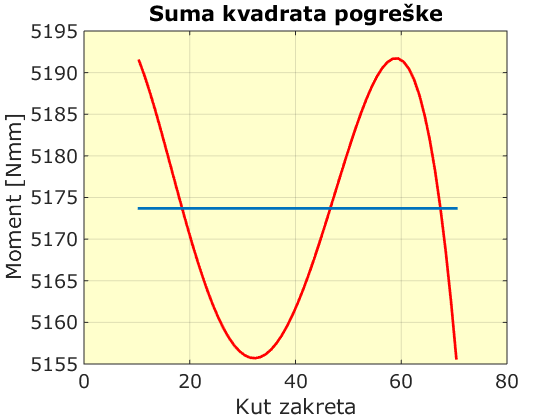
\includegraphics[scale=.6]{slike/max_m1.png}
\caption{Dijagrama odstupanja momenta od traženog (prvi set parametra)}
\label{fig:max_m1}
\end{figure}

\begin{figure}[h!]
\center
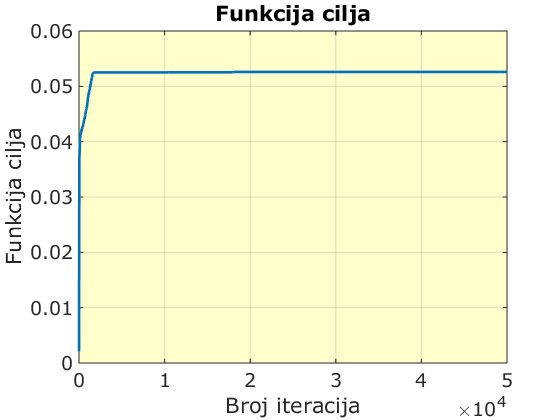
\includegraphics[scale=.6]{slike/max_f1.png}
\caption{Prikaz funkcije cilja (prvi set parametra)}
\label{fig:max_f1}
\end{figure}




\quad Drugi set parametara algoritma dan je sa slijedećim parametrima: 
\begin{itemize}
\item vjerojatnost križanja $0,7$
\item vjerojatnost mutacije $0,01$
\item veličina populacije $100$
\item broj iteracija $10000$
\item funkcija cilja $f(\varphi)=max\left( \mid M_{konst}-M(\varphi)\mid\right) $
\end{itemize}
te su dobiveni su slijedeći rezultati:
\begin{itemize}
\item početne koordinate točke $A(380,28\quad 72,63)$ i točke $B(-137,51\quad  91,57)$ u mm
\item maksimalni moment od $5192,5$  Nmm te minimalni moment od $5154,8$  Nmm
\item vrijednost funkcije cilja $0,0606$
\end{itemize}


Prikaz rezultata za drugi set parametara može se vidjeti na slikama \ref{fig:max_m2} i \ref{fig:max_f2}. Najveća apsolutna razlika u odstupanju od željene vrijednosti momenta iznosi približno $18,8$ Nmm što je vrlo zadovoljavajuće za ovaj mehanizam.

\begin{figure}[h!]
\center
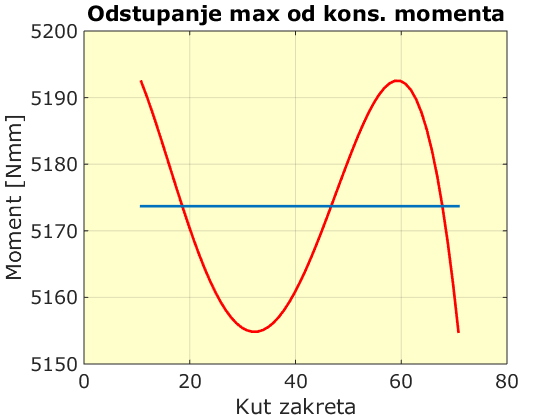
\includegraphics[scale=.6]{slike/max_m2.png}
\caption{Dijagrama odstupanja momenta od traženog (drugi set parametra)}
\label{fig:max_m2}
\end{figure}

\begin{figure}[h!]
\center
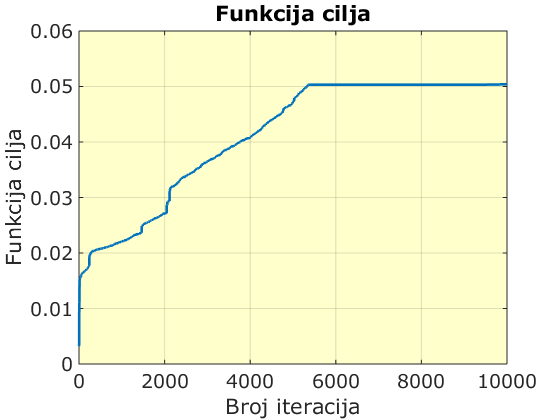
\includegraphics[scale=.6]{slike/max_f2.png}
\caption{Prikaz funkcije cilja (drugi set parametra)}
\label{fig:max_f2}
\end{figure}



\section{Suma kvadrata pogreške}

\quad Treći set parametara algoritma dan je sa slijedećim parametrima: 
\begin{itemize}
\item vjerojatnost križanja $0,7$
\item vjerojatnost mutacije $0,02$
\item veličina populacije $100$
\item broj iteracija $50000$
\item funkcija cilja $f(\varphi)=\sum_{i=1}^{n}\left( M_{konst}-M_i(\varphi) \right)$
\end{itemize}
te su dobiveni su slijedeći rezultati:
\begin{itemize}
\item početne koordinate točke $A(409,21\quad 50)$ i točke $B(-148,88\quad  99,26)$ u mm
\item maksimalni moment od $5182,9$  Nmm te minimalni moment od $5152,3$  Nmm
\item najveća apsolutna razlika u odstupanju od željene vrijednosti iznosi $21,39$ Nmm
\end{itemize}


\begin{figure}[h!]
\center
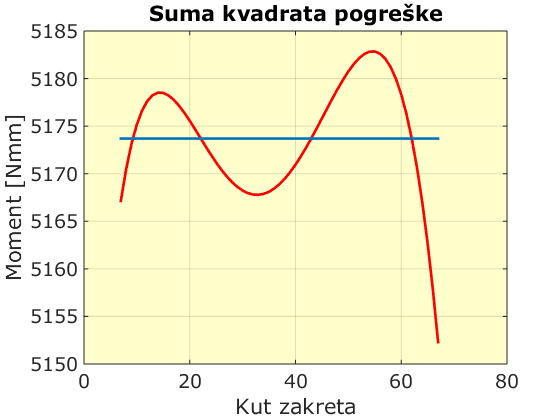
\includegraphics[scale=.6]{slike/sum_m1.png}
\caption{Dijagrama odstupanja momenta od traženog (treći set parametra)}
\label{fig:sum_m1}
\end{figure}

\begin{figure}[h!]
\center
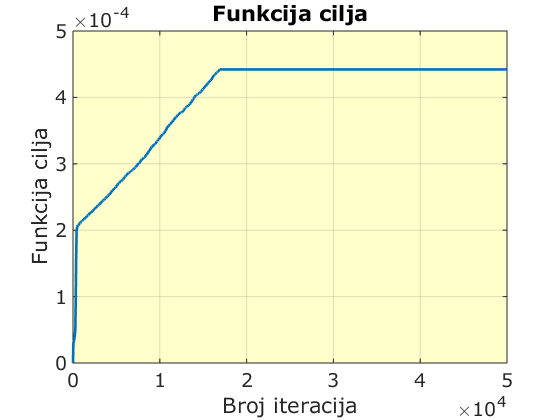
\includegraphics[scale=.6]{slike/sum_f1.png}
\caption{Prikaz funkcije cilja (treći set parametra)}
\label{fig:sum_f1}
\end{figure}



\quad Četvrti set parametara algoritma dan je sa slijedećim parametrima: 
\begin{itemize}
\item vjerojatnost križanja $0,7$
\item vjerojatnost mutacije $0,01$
\item veličina populacije $100$
\item broj iteracija $50000$
\item funkcija cilja $f(\varphi)=\sum_{i=1}^{n}\left( M_{konst}-M_i(\varphi) \right)$
\end{itemize}
te su dobiveni su slijedeći rezultati:
\begin{itemize}
\item početne koordinate točke $A(409,21\quad 50)$ i točke $B(-148,88\quad  99,26)$ u mm
\item maksimalni moment od $5182,9$ Nmm te minimalni moment od $5152,3$  Nmm
\item najveća apsolutna razlika u odstupanju od željene vrijednosti iznosi $21,38$ Nmm
\end{itemize}


\begin{figure}[h!]
\center
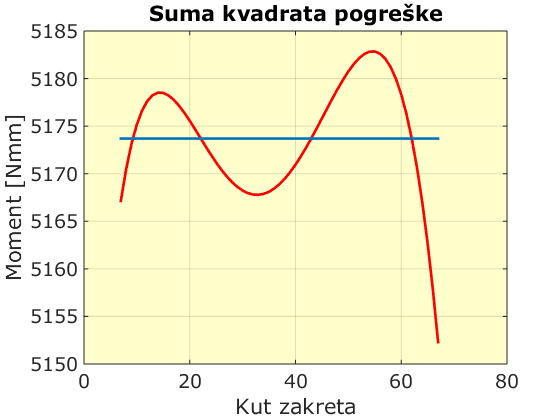
\includegraphics[scale=.6]{slike/sum_m2.png}
\caption{Dijagrama odstupanja momenta od traženog (četvrti set parametra)}
\label{fig:sum_m2}
\end{figure}

\begin{figure}[h!]
\center
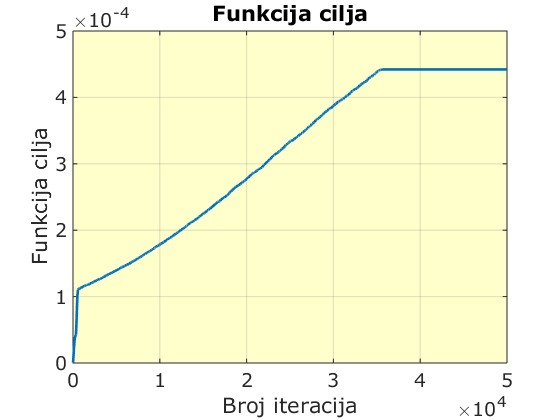
\includegraphics[scale=.6]{slike/sum_f2.png}
\caption{Prikaz funkcije cilja (četvrti set parametra)}
\label{fig:sum_f2}
\end{figure}


Sa slika \ref{fig:sum_m1} i \ref{fig:sum_m2} možemo vidjeti da momentni dijagrama za sumu kvadrata izgledaju isto i imaju iste vrijednosti. Isto tako možemo vidjeti da za vjerojatnost križanja od $0,01$ algoritmu treba puno više iteracija za konvergenciju ka točnom rješenju.



\chapter{Zaključak}
Ovdje ide zaključak rada





% literatura:
\LiteraturaPostavke
\bibliography{literatura}


\appendix
\chapter{Matematički izvodi}
Ovdje ide prilog koji isto moze imati svoju tex datoteku!
Ukoliko je u radu potrebno definirati teorem on se može definirati na slijedeći način:
\begin{theorem}[Proba]
Ovdje ide neki tekst
\begin{equation}
c^2 = a^2+b^2ˇ
\end{equation}
\end{theorem}

Isto vrijedi i za definiciju
\begin{definition}[adf]
Umetni neki tekst
\begin{equation}
c^2 = a^2+b^2ˇ
\end{equation}
\end{definition}



\end{document}





